\section{Features}
\subsection{Pipeline}

\begin{figure}[h]
    \setlength{\unitlength}{0.14in}
    \centering
    \begin{picture}(20,10)
    \put(2,4){\framebox(5,3){\footnotesize{TF}}}
    \put(8,4){\framebox(5,3){\footnotesize{TF-IDF}}}
    \put(14,4){\framebox(5,3){\footnotesize{KBest}}}
    \put(1,1.5){\framebox(19,8){}}
    
    \put(0,5.5){\vector(1,0){2}}
    \put(7,5.5){\vector(1,0){1}}
    \put(19,5.5){\vector(1,0){2}}
    
    \end{picture}
    \caption{Pipeline for the Feature Selection}
    \label{fig:feature-selection}
\end{figure}

\subsection{Term Frequency}

\kaj{Talk about ngrams and show graphs of the comparison of different levels}

\begin{figure*}[ht!]
    \centering
    \subfloat[F1-score for different ngram ranges\label{fig:ngram-f1}]{%
        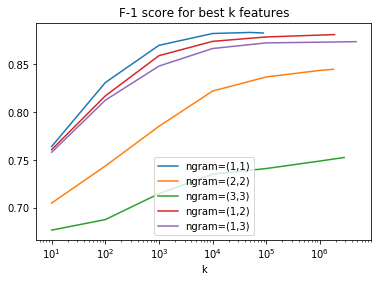
\includegraphics[width=0.3\linewidth]{figures/ngram_range/f1-score.png}}
    \hfill
    \subfloat[Precision-score for different ngram ranges\label{fig:ngram-precision}]{%
        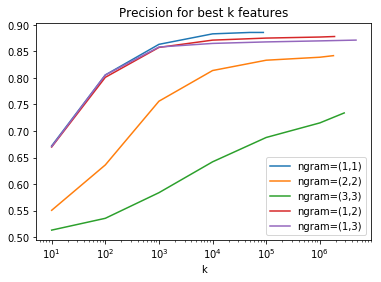
\includegraphics[width=0.3\linewidth]{figures/ngram_range/precision-score.png}}
        \hfill
    \subfloat[Recall-score for different ngram ranges\label{fig:ngram-recall}]{%
        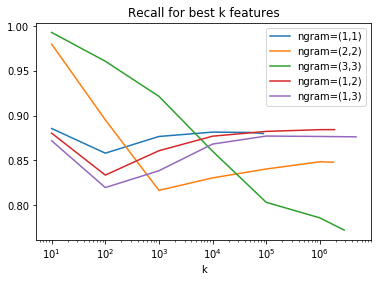
\includegraphics[width=0.3\linewidth]{figures/ngram_range/recall-score.png}}
  \caption{Ngram}
  \label{fig:ngram} 
\end{figure*}

\subsection{Term Frequency- Inverse Document Frequency}


\subsection{Sentiment Analysis}


\subsection{Comparison}

When the three different set of features are compared we can see clearly that TF-IDF is performing best out of the three, closely followed by TF, and on a distance Sentiment analysis using VADER.

\begin{table}
    \centering
    \caption{Results for different features\label{tab:features-comp}}
    \begin{tabular}{ l| S[table-format=1.3] |S[table-format=1.3] |S[table-format=1.3] }
    \hline
        \bf{Feature} & \bf{F1-measure} & \bf{Precision} & \bf{Recall} \\
    \hline
        TF & 0.868 & 0.876 & 0.859 \\ 
        TF-IDF & 0.886 & 0.883 & 0.889 \\
        VADER & 0.719 & 0.716 & 0.721 \\
        \hline
    \end{tabular}
\end{table}
